%\documentclass[12pt,handout]{beamer}
\documentclass{beamer}
\usepackage[ngerman]{babel}
\usepackage[utf8]{inputenc}
\usepackage{amsmath}
\usepackage{amssymb}
\usepackage{listings} 
\usepackage{stmaryrd}
\lstset{language=Python, tabsize=4, showstringspaces=false,basicstyle=\footnotesize,mathescape=true} 
\lstset{literate=%
  {Ö}{{\"O}}1
  {Ä}{{\"A}}1
  {Ü}{{\"U}}1
  {ß}{{\ss}}1
  {ü}{{\"u}}1
  {ä}{{\"a}}1
  {ö}{{\"o}}1
} 
\usepackage{mathtools}
\usepackage{ulem}
\usepackage{tikz}

\usetheme{Boadilla}
\mode<presentation>{
\useoutertheme[subsection=false]{miniframes}
\useinnertheme{rectangles}
%\usecolortheme{crane}
}
\parskip 10pt

\begin{document}
\title{Informatik}   
\author{Suchbaum} 
\date{}
\frame{\titlepage} 

%---
\begin{frame}[fragile]

Ein \textit{binärer Suchbaum}  ist ein binärer Baum, bei dem alle Einträge im linken
Teilbaum eines Knotens x kleiner sind als der Eintrag im Knoten x und bei
dem alle Einträge im rechten Teilbaum eines Knotens x größer sind als der
Eintrag im Knoten x. 

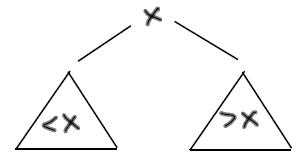
\includegraphics[scale=0.8]{suchbaum1.png} 
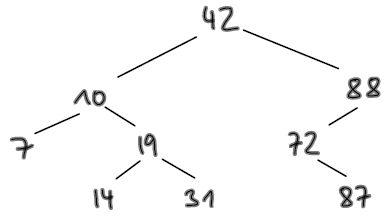
\includegraphics[scale=0.6]{suchbaum2.png} 
\end{frame}

%---
\begin{frame}[fragile]

Methoden des Suchbaums:  

lookup(x): zielgerichtet absteigen und nach x schauen \\ 
~~~ falls gefunden: Verweis liefern,   falls nicht: melden, dass nicht vorhanden  

insert(x): zielgerichtet absteigen und nach x schauen \\ 
~~~~ falls gefunden: melden, dass insert nicht möglich, \\
~~~~  falls nicht gefunden: dort einhängen  

delete(x): zielgerichtet absteigen und nach x schauen  \\
~~~~ falls gefunden: entfernen, \\
~~~~ falls nicht gefunden: melden, dass delete nicht möglich

\end{frame}

%---
\begin{frame}[fragile]


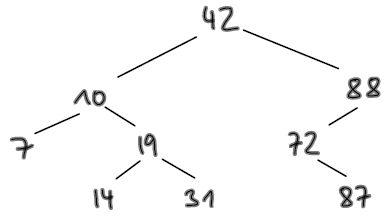
\includegraphics[scale=0.6]{suchbaum2.png}    

lookup 20, 19, 85 \pause 

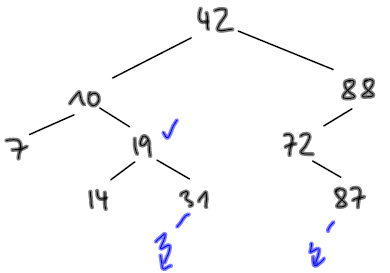
\includegraphics[scale=0.6]{suchbaum3.png}
\end{frame}

%---
\begin{frame}[fragile]
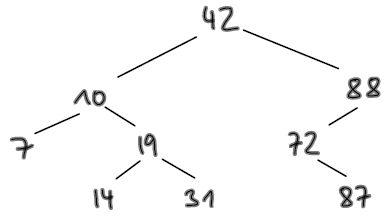
\includegraphics[scale=0.6]{suchbaum2.png}   

insert 5, 18, 70, 71, 20 \pause 

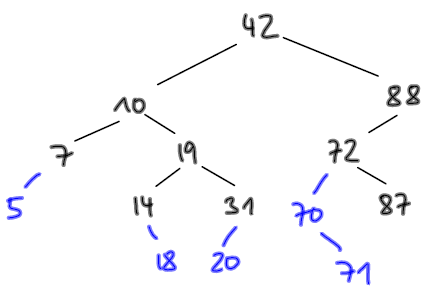
\includegraphics[scale=0.6]{suchbaum4.png}  
 
\end{frame}

%---
\begin{frame}[fragile]
delete 42 - Fall 1: Blatt löschen   

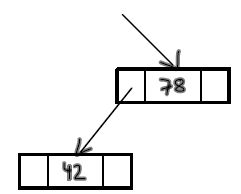
\includegraphics[scale=0.6]{suchbaum8.png}  ~~~~~~  \pause 
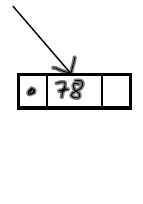
\includegraphics[scale=0.6]{suchbaum9.png}    

delete 42 - Fall 2: ein Sohn  

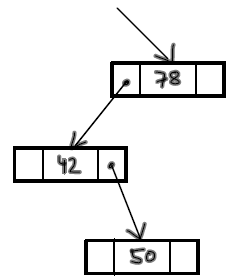
\includegraphics[scale=0.6]{suchbaum10.png}  ~~~~~~  \pause 
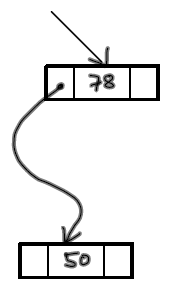
\includegraphics[scale=0.6]{suchbaum11.png}  
 
\end{frame}

%---
\begin{frame}[fragile]
delete 42 - Fall 3: zwei Söhne  

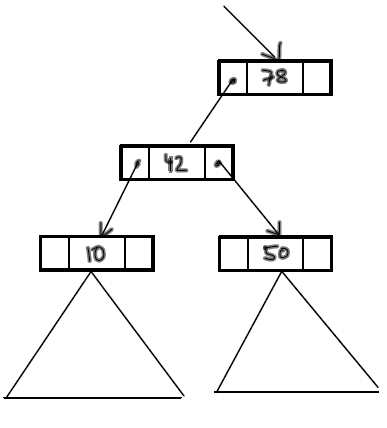
\includegraphics[scale=0.6]{suchbaum12.png}  ~~~~~~ \pause 
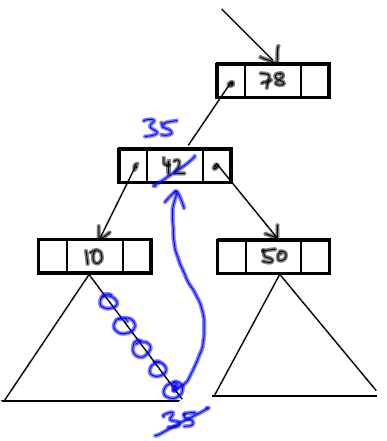
\includegraphics[scale=0.6]{suchbaum13.png}   

Löschen der 35: Fall 1 oder Fall 2.

\end{frame}

%---
\begin{frame}[fragile]
Komplexität der Methoden im Suchbaum: Anzahl Ebenen  

worst case: ~~~~  
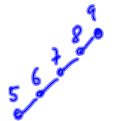
\includegraphics[scale=0.6]{suchbaum6.png}  ~~~~ \pause  O(n)  
 
best case: ~~~~  
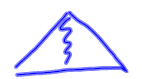
\includegraphics[scale=0.6]{suchbaum7.png}  ~~~~  \pause  O(log(n))   

average case: O(log(n))  
\end{frame}

%---
\begin{frame}[fragile]
\begin{lstlisting}[mathescape=true]
    """
    lookup: 
    Beginne bei der Wurzel
    Solange ein Knoten vorliegt
         vergleiche x mit Knoteninhalt
         steige je nach Vergleich in den linken oder
            rechten Teilbaum ab oder liefere bei
            Gleichheit das Objekt zurück
    Liefere null zurück
    """   $\pause$
    def lookup(self,x):
        k = self.wurzel
        while k is not None:
            if x < k.inhalt:
                k = k.links
            elif x > k.inhalt:
                k = k.rechts
            else:
                return k.inhalt
        return None
\end{lstlisting} 
\end{frame}

%---
\begin{frame}[fragile]
\begin{lstlisting}[mathescape=true]
        
    """
    insert:  
    wenn Baum leer 
         füge neuen Knoten mit x ein 
         melde Erfolg
    sonst
         beginne bei der Wurzel
         solange ein Knoten vorliegt
              merke aktuellen Knoten als Vater
              steige je nach Vergleich in den linken oder
                  rechten Teilbaum ab oder
                  melde bei Gleichheit Mißerfolg
         falls x kleiner als vater
              hänge neuen Knoten links an
         sonst 
              hänge neuen Knoten rechts an
         melde Erfolg
    """    
\end{lstlisting}

\end{frame}

%---
\begin{frame}[fragile]
\begin{lstlisting}
    def insert(self,x):
        if self.wurzel is None:
            self.wurzel = Knoten(x)
            return True
        else:
            vater = None
            k = self.wurzel
            while k is not None:
                vater = k
                if (x < k.inhalt):
                    k = k.links
                elif (x > k.inhalt):
                    k = k.rechts
                else:
                    return False
            if x < vater.inhalt:
                vater.links = Knoten(x)
            else:
                vater.rechts = Knoten(x)
            return True
\end{lstlisting} 
\end{frame}

\begin{frame}[fragile]
Objekte in einen Suchbaum stopfen:

Ist in einer Klasse die magische Methode \texttt{\_\_lt\_\_(self,other)} implementiert, dann wird 
beim Vergleich mit dem Zeichen \texttt{<} diese Methode aufgerufen.

\begin{lstlisting}
class Person:
    def __init__(self,name,alter):
        self.name = name
        self.alter = alter

    def __lt__(self,other):
        return self.name < other.name
\end{lstlisting} 

\end{frame}
 \end{document}